\section{Demonstration by examples}
\label{section:evaluation}

\begin{figure*}[b]
	\centering
	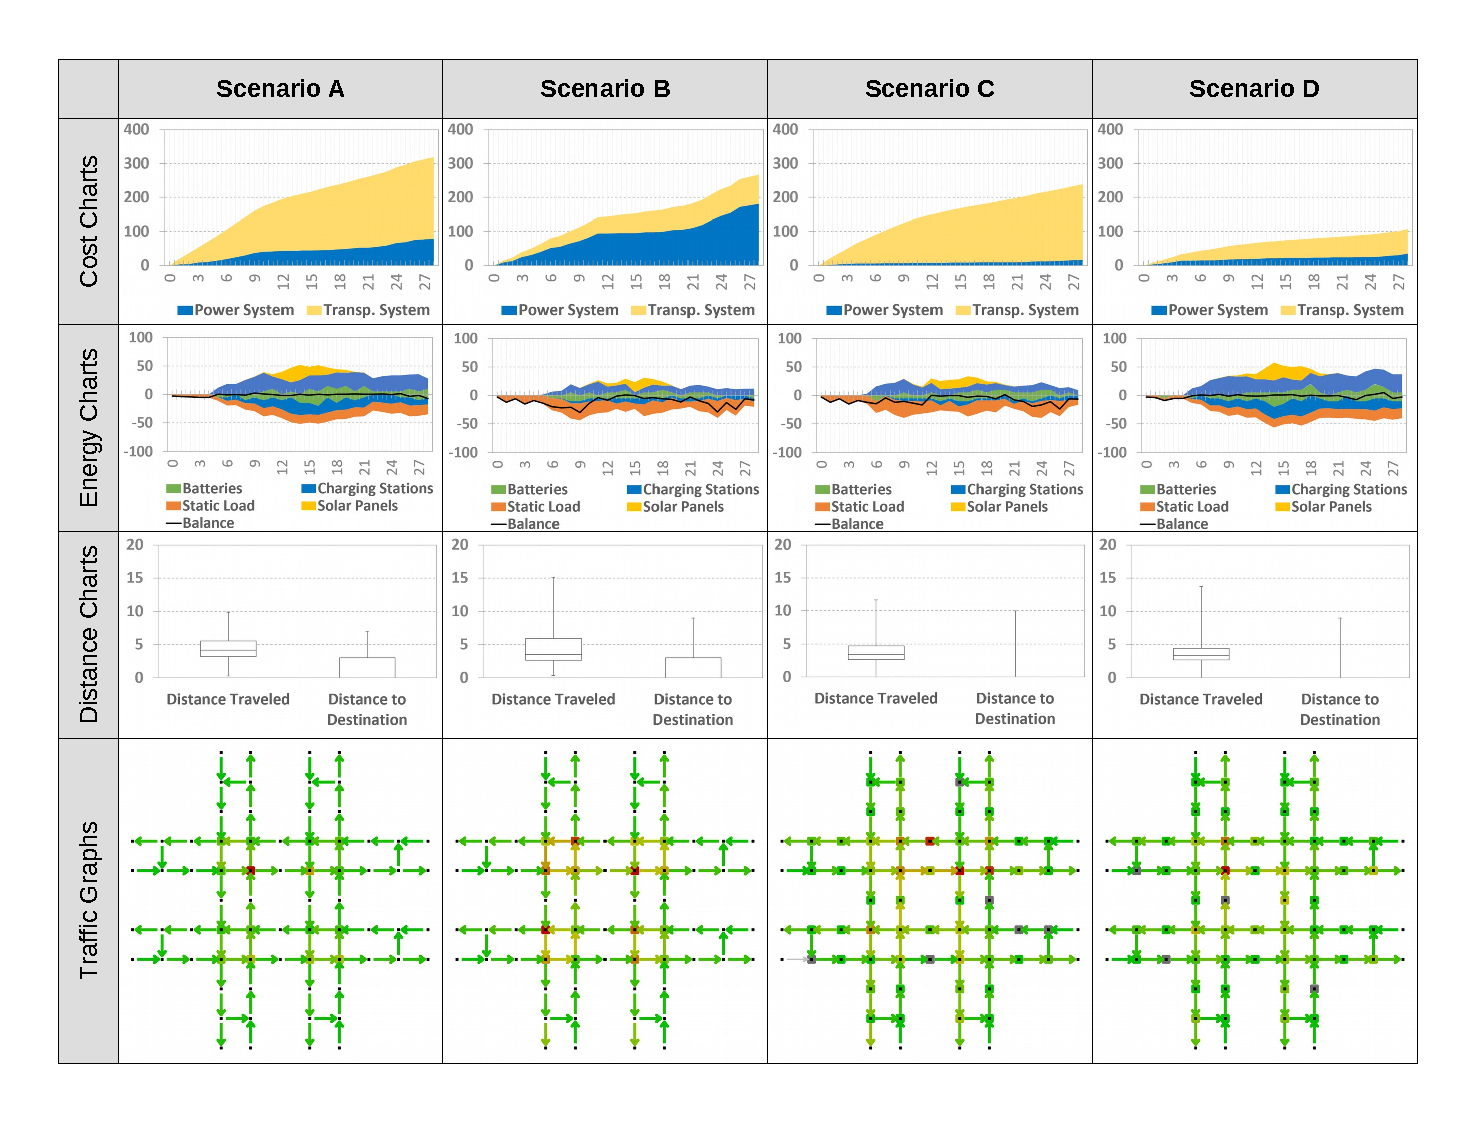
\includegraphics[width=\textwidth]{../gfx/examples2.pdf}
	\caption{Estimated system behavior for all four examples illustrated by energy and cost charts and aggregated traffic graphs.}
	\label{figure:examples}
\end{figure*}

To demonstrate the presented approach, we show a set of different examples with diverse scenario configurations and employed model parameters. Specifically, the proposed examples evaluate the effects of different weight balances between the objectives of the transportation and the power system. 
Furthermore, in the examples, different levels of smart and renewable energy penetration are considered. 

Among all examples, model state is evaluated every 60 seconds to a total of 30 times. This represents a time resolution of 60 seconds with a total observed duration of 30 minutes. 
In terms of aggregated costs, weights of the individual cost functions of power and transportation systems are alternated in the intelligent transportation and power system.

In terms of the power system and it's electric devices, examples include 10 static load components, 5 solar panels, 5 batteries and depending on example, 16 or 56 charging stations. In terms of electricity infrastructure, 4 low voltage nets and 1 medium voltage net are employed. Between examples 1-2 and examples 3-4 power system parameters are varied in terms of the number of charging stations as well as in terms of solar panel and battery capacities. Specifically, the number of charging stations from examples 1 and 2 is increased to the total number of nodes on the traffic network, i.e. 56, in examples 3 and 4. Additionally, from examples 1-2 to examples 3-4, solar panel capacities are increased twofold, while battery capacities are increased fourfold. 

For the transportation system, examples feature a total number of 240 cars. Cars are divided in equal numbers between reference types $C_{A}$, $C_{B}$ and $C_{C}$ with the difference between reference types respectively being state of charge levels at 33\%, 66\% or 99\% of maximum levels. In terms of positioning on the traffic network, origin position of individual cars is randomly drawn from all edges present in the traffic network. Destination positions are randomly drawn from a set of 8 edges of most outward edges of the traffic network. For both origin and destination selection, we employ uniform probabilistic distribution on available options. 

Specifically, differences between the examples for the transportation system and it's subcomponents are described in Table~\ref{tab:example1}. 

\begin{table}[h]
	\renewcommand{\arraystretch}{1.3}
	%\caption{Example Overview}
	\label{tab:example1}
	\centering
	\begin{tabular}{llllll}
		\hline
		\textbf{Parameter/Reference Type}                    & \textbf{Ex. A}    & \textbf{Ex. B} & \textbf{Ex. C} & \textbf{Ex. D}\\ \hline
		Weight Transp. System 			& 0.75	      & 0.25  	& 0.75	& 0.25\\
		Weight Power System 			& 0.25	      & 0.75  	& 0.25	& 0.75\\
		Number Charging Stations              & 16         & 16 		& 56	& 56\\
		Capacity Batteries          & 100 kW/h         & 100 kW/h 		& 400 kW/h		& 400 kW/h\\
		Capacity Solar Panels               & 25 kW/h         & 25 kW/h 		& 50 kW/h		& 50 kW/h	\\ \hline
		Intelligent TS and EN                 & $IS_{A}$         & $IS_{B}$ 		& $IS_{A}$		& $IS_{B}$	\\ 
		Transportation System                 & $TS_{A}$         & $TS_{A}$ 		& $TS_{A}$		& $TS_{A}$	\\ 
		Electric Network                & $EN_{A}$         & $EN_{A}$ 		& $EN_{B}$		& $EN_{B}$	\\ 
		Cars                  & $C_{A,B,C}$          & $C_{A,B,C}$		& $C_{A,B,C}$		& $C_{A,B,C}$	\\ 
		Low Voltage Nets                 & $LV_{A}$         & $LV_{A}$ 		& $LV_{A}$		& $LV_{A}$	\\ 
		Medium Voltage Nets                 & $MV_{A}$         & $MV_{A}$ 		& $MV_{A}$		& $MV_{A}$	\\ 
		Charging Stations                 & $CS_{A}$         & $CS_{A}$ 		& $CS_{A}$		& $CS_{A}$	\\ 
		Power Batteries                & $PB_{A}$         & $PB_{A}$ 		& $PB_{B}$		& $PB_{B}$	\\ 
		Solar Panels                 & $SP_{A}$         & $SP_{A}$ 		& $SP_{B}$		& $SP_{B}$	\\ 
		Static Loads                 & $SL_{A}$         & $SL_{A}$ 		& $SL_{B}$		& $SL_{B}$	\\ \hline
	\end{tabular}
\end{table}

\subsection*{Scenario 1: Prefer transportation, low penetration}
Example 1 describes a scenario with a low number and low capacities of smart and renewable energy devices. That is, low solar panel capacity, low battery capacity is available and static profile simulating net influence has high impact. Also, only a low number of charging stations is available for cars. More weight is put on the costs incurred by transportation instead of the power system, in benefit of achieving the objectives of the transportation system. Behavior estimation results show low frequency of edges around and on charging stations. Furthermore, net balance is prone to high and sudden fluctuations in load. Little equalization of negative net balances is made by cars discharging at charging stations. In result, incurred transportation system costs are very high, while power system costs are low.

\subsection*{Scenario 2: Prefer power, low penetration}

In Example 2, numbers and capacities of smart and renewable energy devices are equal to Example 1. However, different to Example 1, more weight is put on the costs incurred by power system instead of the transportation system, in benefit of achieving the objectives of the power system. Behavior estimation results show higher frequency of edges around and on charging stations compared to example 1. Also in contrast to Example 1, net negative balances are equalized more heavily, which can be traced to cars discharging at charging stations. While energy capacity of storages and solar panels is low and load balancing only occurs to small degree, balancing is more heavily utilized compared to Example 1. Due to objective weight, costs of the power system are higher than in example 1, but in combination with the transportation system, lower total costs are achieved.

\subsection*{Scenario 3: Prefer transportation, high penetration}

In Example 3, smart and renewable energy penetration is increased through additional solar panel and battery capacity as well as a higher number of charging stations distributed on the traffic network. Also, the profile of static loads is more evened out, as the power grid and it's electric devices get more smart resulting in a less power load peaks. 
Equal to example 1, more weight is put on the costs incurred by transportation instead of the power system, in benefit of achieving the objectives of the transportation system. Behavior estimation results show low frequency of edges around and on charging stations. Furthermore, net balance is prone to high and sudden fluctuations in load. Equalization of negative net balances is seen by higher capacities of solar panels and batteries as well as a higher number of charging stations, in contrast to Examples 1 and 2. In result, costs are much lower compared to examples 1 and 2.

\subsection*{Scenario 4: Prefer power, high penetration}

In Example 4, numbers and capacities of smart and renewable energy devices are equal to Example 3. Different to example 3, weight of power system costs is greater than weight of transportation system costs. Behavior estimation results show higher frequency of edges around and on charging stations compared to example 3, however, compared to example 2, frequency is distributed more evenly across the traffic network. In contrast to Example 3, negative net balances are equalized more evenly. In result, this leads to very low power system and low transportation system costs.